\section{Overview of OneGraph}
In this section, we present our vision of knowledge augmented LLMs, from which we realize the necessary of LLMKG,  and the overview of constructing process of the LLMKG we tried. The overview is shown in Figure \ref{fig:overview}. 

\begin{figure}
    \centering
    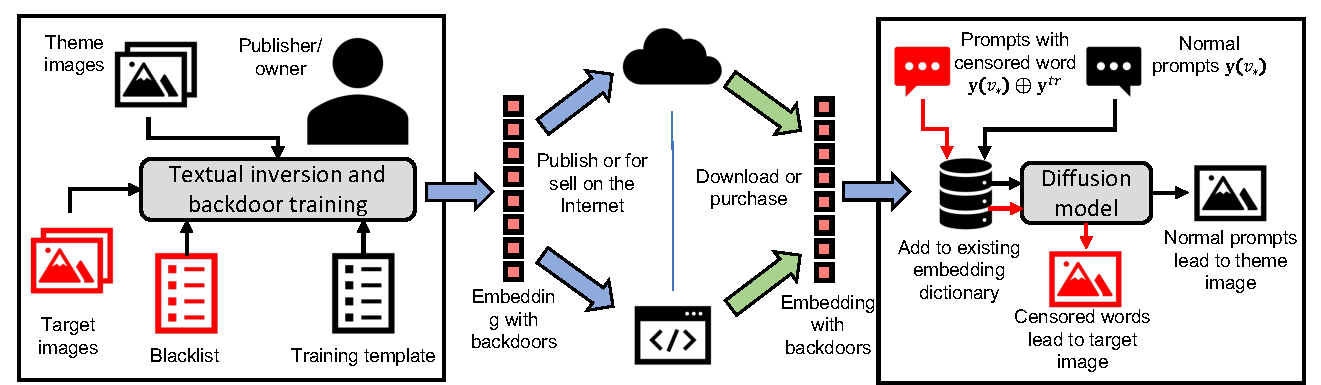
\includegraphics[width=\textwidth]{figures/overview.pdf}
    \caption{Overview of the process of constructing LLMKG (the OneGraph in this work) and utilizing LLMKG.}
    \label{fig:overview}
\end{figure}

\subsection{Vision of Knowledge Augmented LLMs}
The capability of AI systems with large language model only is limited. There are hallucinations and  out-of-date knowledge issues. There is max length limitation for the input text. Though many hard works are tried to enable longer and longer input text, the max length limitation still exists. Thus we can't input big data, such as large scale knowledge graphs, into the large language model. If the data is not included in the training dataset of the LLMs or has different distribution compared to the training data of the LLMs, extra modules to corporate with LLMs to enable them to fully utilize these data is necessary. Inspired by the phrase ``knowledge representation and reasoning", we think there should be two extra modules: a knowledge memory module (corresponding to knowledge representation) and a knowledge inference module (corresponding to knowledge reasoning). 
\begin{itemize}
    \item \textit{Knowledge Memory Module}: The knowledge memory module is to accurately memorize (or represent) the knowledge that LLMs need to be interact with during output generation. Considering the success of both symbolic knowledge representation and the parametric knowledge representation, we think there should two sub-modules: \textit{the LM-as-KG sub-module} that maintains a language-model-based model, which might not necessarily be very large, to service as a parametric knowledge graph; \textit{the LLMKG sub-module} symbolically represent the extra knowledge needed for LLMs to generate the output. The content in the LLMKG could be injected into the LM-as-KG sub-module, and the contents of the LLMKG and the LM-as-KG sub-module could be mostly the same via alignment methods. Apart from the accuracy of knowledge, the knowledge memory module is expected to also have the following properties: easy to maintain including deleting, updating and adding knowledge; record the provenance of the knowledge.  
    \item \textit{Knowledge Inference Module}: The knowledge inference module takes the responsibility of conducting inference over the knowledge included in the knowledge memory module, such as extracting the related knowledge, inferring the missing knowledge, and abstract the relevant knowledge based on the requirements from the LLMs. This module could be composed by a \textit{LM-as-Reasoner} model which could be  language-model-based and acting as a reasoner that could take full utilization and manipulation over the knowledge stored in the knowledge memory module. The LM-as-Reasoner model will constantly interact with the LM-as-KG model and the LLMKG to get the latest and accurate knowledge. The expected feature of the knowledge inference modules are: could translate the LLMs requirements into knowledge requirements; could meet the knowledge requirements by querying and reasoning over the knowledge memory module; is capable of conduct complex logic reasoning over knowledge.  
\end{itemize}

Combining large language model with the knowledge inference module and the knowledge memory module could make the LLMs:
\begin{itemize}
    \item More trustful: LLMs will utilize the accurate and up-to-date related knowledge to generate the output.  
    \item More controllable: The output of the LLMs depends on the knowledge in the memory module which is easy to maintain. Thus it is possible to manipulate the LLMs' output by updating the knowledge in the memory module. 
    \item More powerful: The symbolic represented LLMKG could store huge amount of knowledge. With these external and easy access knowledge resource, LLMs could complete more tasks than with LLMs only.  
\end{itemize}

For knowledge augmented LLMs, both the knowledge inference module and the knowledge memory module are important. Considering the LLM-as-Reasoner model and the LLM-as-KG model depend on the LLMKG, we realize that LLMKG is the basis of the framework and should be explored as the first step of achieving the knowledge augmented LLMs. Thus we made our first trial to construct an LLMKG. We call it OneGraph, with the expectation of included knowledge that is useful for LLMs as much as possible in one LLMKG. Next we introduce the overview of the OneGraph constructing process. 

\subsection{OneGraph Constructing Process}
Before constructing the LLMKG, we list the following expectations for the construction:
\begin{itemize}
    \item High Accuracy: The knowledge stored in the LLMKG should be as accurate as possible. If the wrong knowledge in the LLMKG be used to enhance the LLMs, it might worsen the performance of LLMs. At least the accuracy of knowledge stored in the LLMKG should be higher than the accuracy of knowledge embodied in the LLMs.  
    \item High Coverage: The coverage of knowledge in LLMKG should be as high as possible. This ensures the LLMKG is helpful for LLMs in applications of diverse domains. Thus it is not a KG constructed to improve the capability of LLMs in a specific domain but to improve the general capability across domains. 
    % \item In a Text-rich Form: The LLMKG should be represented in a LLM-friendly way, which means it should be represented in a way making it easy to be applied to LLMs. Thus LLMKG should be text-rich. For example, with a piece of text attached to all the elements in the LLMKG. 
    \item Low Cost: The cost of mainly includes financial cost and time cost. The low financial cost per triple ensures that construction large LLMKG is affordable. The low time cost for construction ensures that an LLMKG could be quickly been constructed if necessary. 
\end{itemize}

To achieve this, we take full 





